% Credit goes to:
% Adrien Friggeri and Carmine Benedetto whose FancyCV and SmartFancyCV are the basis for my work:
	% https://github.com/neoben/smart-fancy-latex-cv/commits?author=neoben
%!TEX TS-program = XeLaTex / XeLaTex + MakeIndex
%Most of Doug´s data courtesy of https://kingofqueens.fandom.com

\documentclass[]{friggeri-cv_reccius-experiment}
\usepackage{afterpage}
\usepackage{hyperref}
\usepackage{color}
\usepackage{xcolor}
\PassOptionsToPackage{cmyk}{xcolor}
\usepackage{smartdiagram}
\usepackage{fontspec}
\usepackage{fontawesome}
\usepackage{marvosym}
\usepackage{textcomp}
\usepackage{float} % to position signature
\usepackage{adjustbox}
\usepackage{calc}
\usepackage{enumitem} % to customize indent of bullet points via \itemize
\usepackage{metalogo}
\usepackage{dtklogos}
\usepackage[utf8]{inputenc}
\usepackage{tikz}
\usetikzlibrary{mindmap,shadows,positioning}
\hypersetup{
    pdftitle={},
    pdfauthor={},
    pdfsubject={},
    pdfkeywords={},
    colorlinks=false,           % no lik border color
    allbordercolors=white       % white border color for all
}
\smartdiagramset{
    bubble center node font = \footnotesize,
    bubble node font = \footnotesize,
    % specifies the minimum size of the bubble center node
    bubble center node size = 0.06cm,
    %  specifies the minimum size of the bubbles
    bubble node size = 0mm,
    % specifies which is the distance among the bubble center node and the other bubbles
    distance center/other bubbles = 0.8cm,
    % sets the distance from the text to the border of the bubble center node
    distance text center bubble = 0.3cm,
    % set center bubble color
    bubble center node color = centergray,
    % define the list of colors usable in the diagram
    set color list = {bubblegray, bubblegray, bubblegray, bubblegray, bubblegray, white, lightgray, lightgray, lightgray, lightgray},
    % sets the opacity at which the bubbles are shown
    bubble fill opacity = 0.7,
    % sets the opacity at which the bubble text is shown
    bubble text opacity = 1,
}

% \addbibresource{bibliography.bib}
\RequirePackage{xcolor}
\definecolor{lightgray}{HTML}{777788}
\definecolor{centergray}{HTML}{B9B9C9}
% you can change ipsgreen to any color you like, but you´ll also have to change it in the reccius-cv-experiment.cls file
\definecolor{ipsgreen}{HTML}{3B6746}

% NAME AND TAGLINE
\begin{document}
\header{Doug}{Heffernan}
      {Passionate Driver}

\vspace{0.3cm}
\color{lightgray}\noindent\makebox[\textwidth]{\rule{\paperwidth-0.4cm}{2.5pt}}
% In the aside, each new line forces a line break

%%%%%%%%%%%%%%%%%%%%%%%%%%%%%%%%%%%%%
%%%%%%%%%%%%                 CONTACT                %%%%%%%%%%
%%%%%%%%%%%%%%%%%%%%%%%%%%%%%%%%%%%%%

\begin{info}
    \begin{flushleft}
    {{\small February 9, 1965}\hfill{\LARGE \textborn\thinspace\thinspace\verythinspace}\\

    \vspace{0.11cm}

    \small 3121 Aberdeen Road, Queens, NY}\hfill{\Large\faMapMarker\thinspace\thinspace\thinspace}\\

    \vspace{0.08cm}

    {\small (718) 555-LOGS}\hfill{\LARGE\Mobilefone\thinspace}\\

    \vspace{0.14cm}

    \href{mailto:doug.heffernan@international-parcel-service.com}{{\small\textbf{doug.heffernan@}ips-nyc.com}\hfill{\Large\Letter}\hspace{0.6mm}{\small \faMousePointer}}\\

    \end{flushleft}
\end{info}

%%%%%%%%%%%%%%%%%%%%%%%%%%%%%%%%%%%
%%% %%%%%%%%               SIDE BARS               %%%%%%%%%
%%%%%%%%%%%%%%%%%%%%%%%%%%%%%%%%%%%
\begin{aside}
    ~

% PICTURE
\vspace{-3.5cm}
\begin{figure}[ht]
	\hspace{0.3cm}
	\includegraphics[width=.71\linewidth]{img/Doug.png}
\end{figure}

% SKILLS
\newcommand{\skillspace}{\vspace*{-0.75mm}}
  \vspace{-2.9mm}
  \section{Skills\thinspace \&\thinspace Strengths}\\
  \vspace{3.5mm}

	\textbf{Driving}\\\vspace{0.4mm}
	\begin{itemize}[leftmargin=*, noitemsep]
	\item Save and punctual delivery of packages to end consumers
	\item Rudimentary vehicle maintenance task\\
	\end{itemize}

  	\skillspace
    	\textbf{People Skills}\\\vspace{0.2mm}
	\begin{itemize}[leftmargin=*, noitemsep]
	\item Contributes significantly to collegial athmosphere\\
	\end{itemize}

  	\skillspace
	\textbf{BBQ}\\\vspace{0.4mm}
	\begin{itemize}[leftmargin=*, noitemsep]
	\item Your steaks, your bacons, your bratwursts \\
	\item Definitely no tofu! \\
	\end{itemize}

  	\skillspace
	\textbf{Athletics}\\\vspace{0.2mm}
	\begin{itemize}[leftmargin=*, noitemsep]
	\item Tried out for Nassau Rebels semi-pro football team twice\\
	\end{itemize}

  	\skillspace
	\textbf{Caregiving}\\\vspace{0.4mm}
	\begin{itemize}[leftmargin=*, noitemsep]
	\item Providing home (basement) for father-in-law for years\\
	\end{itemize}

    \vspace{0.5mm}
    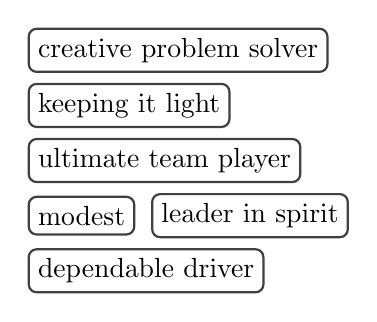
\begin{tikzpicture}[node distance = 7mm, terminal/.style={
    	rectangle, minimum height = 2mm, rounded corners = 1mm, thick,
    	draw = darkgray, fill = white, align = left}]
    	\node (A) [terminal] {creative problem solver};
    	\node (B) [terminal, below=of A.west,anchor=west] {keeping it light};
    	\node (C) [terminal, below=of B.west,anchor=west] {ultimate team player};
    	\node (D) [terminal, below=of C.west,anchor=west] {modest};
    	\node (E) [terminal, right=2mm of D.east,anchor=west] {leader in spirit};
    	\node (F) [terminal, below=of D.west,anchor=west] {dependable driver};
	\end{tikzpicture}

  \vspace{-2.6mm}
  \section{Eager to deepen knowledge about...}\\
  	\begin{itemize}[leftmargin=*, noitemsep]
	\vspace{3mm}
	\item ...baloney-darts
	\item ...getting back into shape
	\item ...containing cranky old people
	\end{itemize}

  \vspace{-2.7mm}
  \section{Sports Teams}\\
  \vspace{1.0mm}
  \smartdiagram[bubble diagram]{
  	  \hspace{-5.5mm}
        \includegraphics[width=13mm]{img/NFL.png}\\\vspace{1mm}
        {\small\textbf{5/5}}
        ,
        \includegraphics[width=14.5mm]{img/Jets.png}\\
        \textbf{4/5}
        ,
        \includegraphics[width=13mm]{img/Mets.png}\\
        \textbf{5/5}
        ,
        \includegraphics[width=13mm]{img/Islanders.png}\\
        \textbf{4/5}
        ,
        \includegraphics[width=15mm]{img/Patriots.png}\\
        \textbf{-6/5}
        ,
        \includegraphics[width=12.5mm]{img/Knicks.png}\\
        \textbf{4/5}}
\end{aside}
~
% LANGUAGES
\newcommand{\belowspace}{\vspace*{0.85mm}}
\begin{below1}
  \section{Languages}
    \\\vspace{1.7mm}
    \textbf{English}\hfill
    \includegraphics[scale=0.11]{img/IPSGreenDots.png}
    \includegraphics[scale=0.11]{img/IPSGreenDots.png}
    \includegraphics[scale=0.11]{img/IPSGreenDots.png}
    \includegraphics[scale=0.11]{img/IPSGreenDots.png}
    \includegraphics[scale=0.11]{img/IPSGreenDots.png}
    \includegraphics[scale=0.11]{img/IPSGreenDots.png}\\
    \belowspace
    \textbf{Japanese}\hfill
    \includegraphics[scale=0.11]{img/IPSGreenDots.png}
    \includegraphics[scale=0.11]{img/IPSGreenDots.png}
    \includegraphics[scale=0.11]{img/WhiteDots.png}
    \includegraphics[scale=0.11]{img/WhiteDots.png}
    \includegraphics[scale=0.11]{img/WhiteDots.png}
    \includegraphics[scale=0.11]{img/WhiteDots.png}\\
    \belowspace
    \textbf{Spanish}\hfill
    \includegraphics[scale=0.11]{img/IPSGreenDots.png}
    \includegraphics[scale=0.11]{img/WhiteDots.png}
    \includegraphics[scale=0.11]{img/WhiteDots.png}
    \includegraphics[scale=0.11]{img/WhiteDots.png}
    \includegraphics[scale=0.11]{img/WhiteDots.png}
    \includegraphics[scale=0.11]{img/WhiteDots.png}\\
    \belowspace
    \textbf{French}\hfill
    \includegraphics[scale=0.11]{img/IPSGreenDots.png}
    \includegraphics[scale=0.11]{img/WhiteDots.png}
    \includegraphics[scale=0.11]{img/WhiteDots.png}
    \includegraphics[scale=0.11]{img/WhiteDots.png}
    \includegraphics[scale=0.11]{img/WhiteDots.png}
    \includegraphics[scale=0.11]{img/WhiteDots.png}\\~
\end{below1}

% INTERESTS
\begin{below2}
  \section{Interests \& Activities}
    \\\vspace{1.7mm}
    \textbf{Football (watching, occasionally playing) | Rock Music |\\
    \belowspace
    Bruce Springsteen | Good Food} \\
    \belowspace
    \textbf{Bowling}\hfill\href{https://kingofqueens.fandom.com/wiki/Doug_Heffernan}{\small Cooper´s Onion Ringers} since 1999\\
    \belowspace
    \textbf{Softball}\hfill\href{https://kingofqueens.fandom.com/wiki/Doug_Heffernan}{\faMousePointer}\thinspace \thinspace board member\thinspace from\thinspace 1998-1999\\

~
\end{below2}
%%%%%%%%%%%%%%%%%%%%%%%%%%%%%%%%%%%
%%% %%%%%%%%             EDUCATION             %%%%%%%%%%
%%%%%%%%%%%%%%%%%%%%%%%%%%%%%%%%%%%
\newcommand{\eduspace}{\vspace*{0.85mm}}
\newcommand{\eduspaceII}{\vspace*{0.8mm}}
\newcommand{\jobspace}{\vspace*{-4.2mm}}
\vspace{-0.5mm}

\section{EDUCATION}
\begin{entrylist}

   \entry
    {March, 2005\enspace}
    {Advanced Training | }{\small{internal}}
    {\normalsize\textbf{\color{ipsgreen}\faMapMarker\space International Parcel Service (IPS)}}
    {\jobspace
    \begin{itemize}[leftmargin=*, itemsep = 0.1em]
    \item Completed the IPS aptitude test for aspiring managerial staff
    \item Subsequently decided to keep pursuing his passion for driving and delivering instead\\
    \end{itemize}}

  \entry
    {1985 - 1986\enspace}
    {Junior College | }{\small{no degree}}
    {\normalsize\textbf{\color{ipsgreen}\faMapMarker\space Nassau Community College}}
    {\textbf{Coursework:} \\College Preparatory English, Introduction to College Biology I, Contemporary Music, The History of Sports in America
    \eduspace\\}

  \entry
    {1980 - 1984\enspace}
    {High School Diploma | } {\Large\diameter\thinspace\normalsize 1.7 GPA}
    {\normalsize\textbf{\color{ipsgreen}\faMapMarker\space St. Gregory's High School, Queens, NY}
    }
    {\textbf{Honors Classes}: \\Physical Education, running back (All-County)}\vspace{-2.8mm}
\end{entrylist}
%%%%%%%%%%%%%%%%%%%%%%%%%%%%%%%%%%
%%%%%%%%%%%%       EXPERIENCE       %%%%%%%%%%%%
%%%%%%%%%%%%%%%%%%%%%%%%%%%%%%%%%%
\section{EXPERIENCE}
\begin{entrylist}

  \entry
    {1994 - now\enspace}
    {Truck Driver | }{ \href{https://kingofqueens.fandom.com/de/wiki/International_Parcel_Service}{\small Queens Area \faMousePointer}}
    {\normalsize\textbf{\color{ipsgreen}\faMapMarker\space International Parcel Service (IPS)}}
    {\jobspace
    \begin{itemize}[leftmargin=*, itemsep = 0.1em]
    \item Delivered packages to costumers around New York City (mostly Queens)
    \item Practiced solidarity as a union member during a driver strike in the year 2000
    \item Occasionally chosen to move specialty items such as live animals between NY Zoos
    \item Company-wide record holder for \textit{number of days without an "incident" - no complaints or broken packages}
    \item Was profiled in the company newsletter \textit{IP-Yes}\\
    \end{itemize}
    }

  \entry
    {May, 1999\enspace}
    {Interim Shift Supervisor | }{ \href{https://kingofqueens.fandom.com/de/wiki/International_Parcel_Service}{\small Queens Office \faMousePointer}}
    {\normalsize\textbf{\color{ipsgreen}\faMapMarker\space International Parcel Service (IPS)}}
    {\jobspace
    \begin{itemize}[leftmargin=*, itemsep = 0.1em]
    \item Brief detour into white collar occupation when the team was in need
    \item Provided temporary support to the office in the absense of supervisor O´Boyle (personal leave of absense)
    \item Scheduled routes for drivers
    \item Managed the budget
    \item Contributed to the motivation of all drivers and loaders\\
    \end{itemize}
    }

  \entry
    {1992\,-\,1993\enspace}
    {Truck Loader | }{\href{https://kingofqueens.fandom.com/de/wiki/International_Parcel_Service}{\small Packages \& Cargo \faMousePointer}}
    {\normalsize\textbf{\color{ipsgreen}\faMapMarker\space International Parcel Service (IPS)}}
    {\jobspace
    \begin{itemize}[leftmargin=*, noitemsep]
    \item Loaded all packages securely and in a logical order for the drivers to deliver
    \item Worked closely with the drivers to ensure maximum efficiency and safety
    \item Briefly returned to loading duties due to an unfortunate test-taking incident in 2002 \\
    \end{itemize}
    }

  \entry
    {1988\,-\,1991\enspace}
    {Security Guard  | }{\small Nightclub \& Bar}
    {\normalsize\textbf{\color{ipsgreen}\faMapMarker\space Sour Polly, Queens, NY}}
    {\jobspace
    \begin{itemize}[leftmargin=*, itemsep = 0.1em]
    \item Providing rigorous access control of costumers
    \item Making difficult and critical entry decisions
    \item Keeping the customers safe and entertained\\
    \end{itemize}
    }

\end{entrylist}

% SIGNATURE
\vspace{-12.5mm}
\begin{figure}[H]
\hspace{11cm}
\includegraphics[scale=0.5]{img/KevinJamesSignature.jpg}
\end{figure}
\vspace{-1.05cm}
\hspace{6.5cm} Queens, NY, May 14th, 2007
\end{document}
